\resetfigpath{2-datasets}
\chapter{Datasets}

\label{datasets} % For referencing the chapter elsewhere, use \ref{Chapter1}

This chapter first describes the dataset modalities and properties.
Second, we give an overview of our pipeline from training to evaluation.
Third, we introduce the proposed methods for feature learning as well as the evaluation scheme.
Concerning the feature representation learning, we first introduce our baseline methods, followed by the U-Net based methods.

Tab. \ref{tab:dataset_stat} summarizes the 13 datasets. We used four different MRI brain sequences (A-D). To augment the number of images for one dataset, the last three datasets (B-D) are combined into one larger dataset \textit{MRI Brain (B-D)}. In a similar manner, dataset \textit{Slit-Lamp Retina (A-D)} is constructed from concatenating four independent datasets together. The two independent datasets of the inner ear CT could not be concatenated due to different image resolutions. To each dataset, we also have corresponding xy-coordinates of the gaze location.

\begin{table}[ht]
   \centering
   \caption[Dataset statistics]{Summary and statistics of used datasets.}
   \begin{tabular}{l|c|c|c|c|c}
      \toprule
      \textbf{Name} & \textbf{Size $N$} & \textbf{Height $H$ [px]} & \textbf{Width $W$ [px]} & \textbf{\#Channels $C$} \\
      \midrule
      Surgical Video Sequence & 1125 & 576 & 720 & 3 - RGB \\
      \midrule
      MRI Brain A & 129 & 540 & 782 & 1 - Gray \\
      MRI Brain B & 69 & 512 & 680 & 1 - Gray \\
      MRI Brain C & 75 & 512 & 680 & 1 - Gray \\
      MRI Brain D & 75 & 512 & 680 & 1 - Gray \\
      MRI Brain (B-D) & 219 & 512 & 680 & 1 - Gray \\
      \midrule
      CT Inner Ear A & 96 & 191 & 252 & 1 - Gray \\
      CT Inner Ear B & 99 & 290 & 300 & 1 - Gray \\
      \midrule
      Slit-Lamp Retina A & 194 & 512 & 680 & 3 - RGB \\
      Slit-Lamp Retina B & 121 & 512 & 680 & 3 - RGB \\
      Slit-Lamp Retina C & 75 & 512 & 680 & 3 - RGB \\
      Slit-Lamp Retina D & 130 & 512 & 680 & 3 - RGB \\
      Slit-Lamp Retina (A-D) & 520 & 512 & 680 & 3 - RGB \\
      \bottomrule
   \end{tabular}
   \label{tab:dataset_stat}
\end{table}

\begin{figure}[t!]
\centering
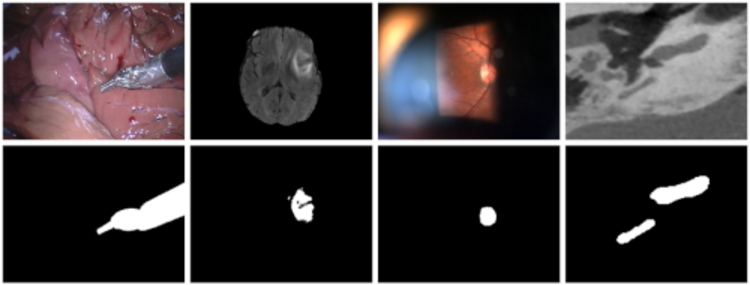
\includegraphics[width=0.99\textwidth]{previews.pdf}
\caption{Example of objects of interest in different video and volumetric modalities. The bottom row shows the pixel wise segmentation for each case: From left to right: A surgical instrument during an endoscopic procedure, a 3D MRI scan containing a brain tumor, an optic disc seen from a slit lamp microscope and a cochlea cross-section in a 3D CT scan.}
\label{fig:dset_previews}
\end{figure}

%%% Local Variables:
%%% mode: latex
%%% TeX-master: "../../main"
%%% End:
